\section{实验结果及分析}
\begin{figure}[H]
  \centering

  \begin{subfigure}[b]{0.6\textwidth}
    \centering
    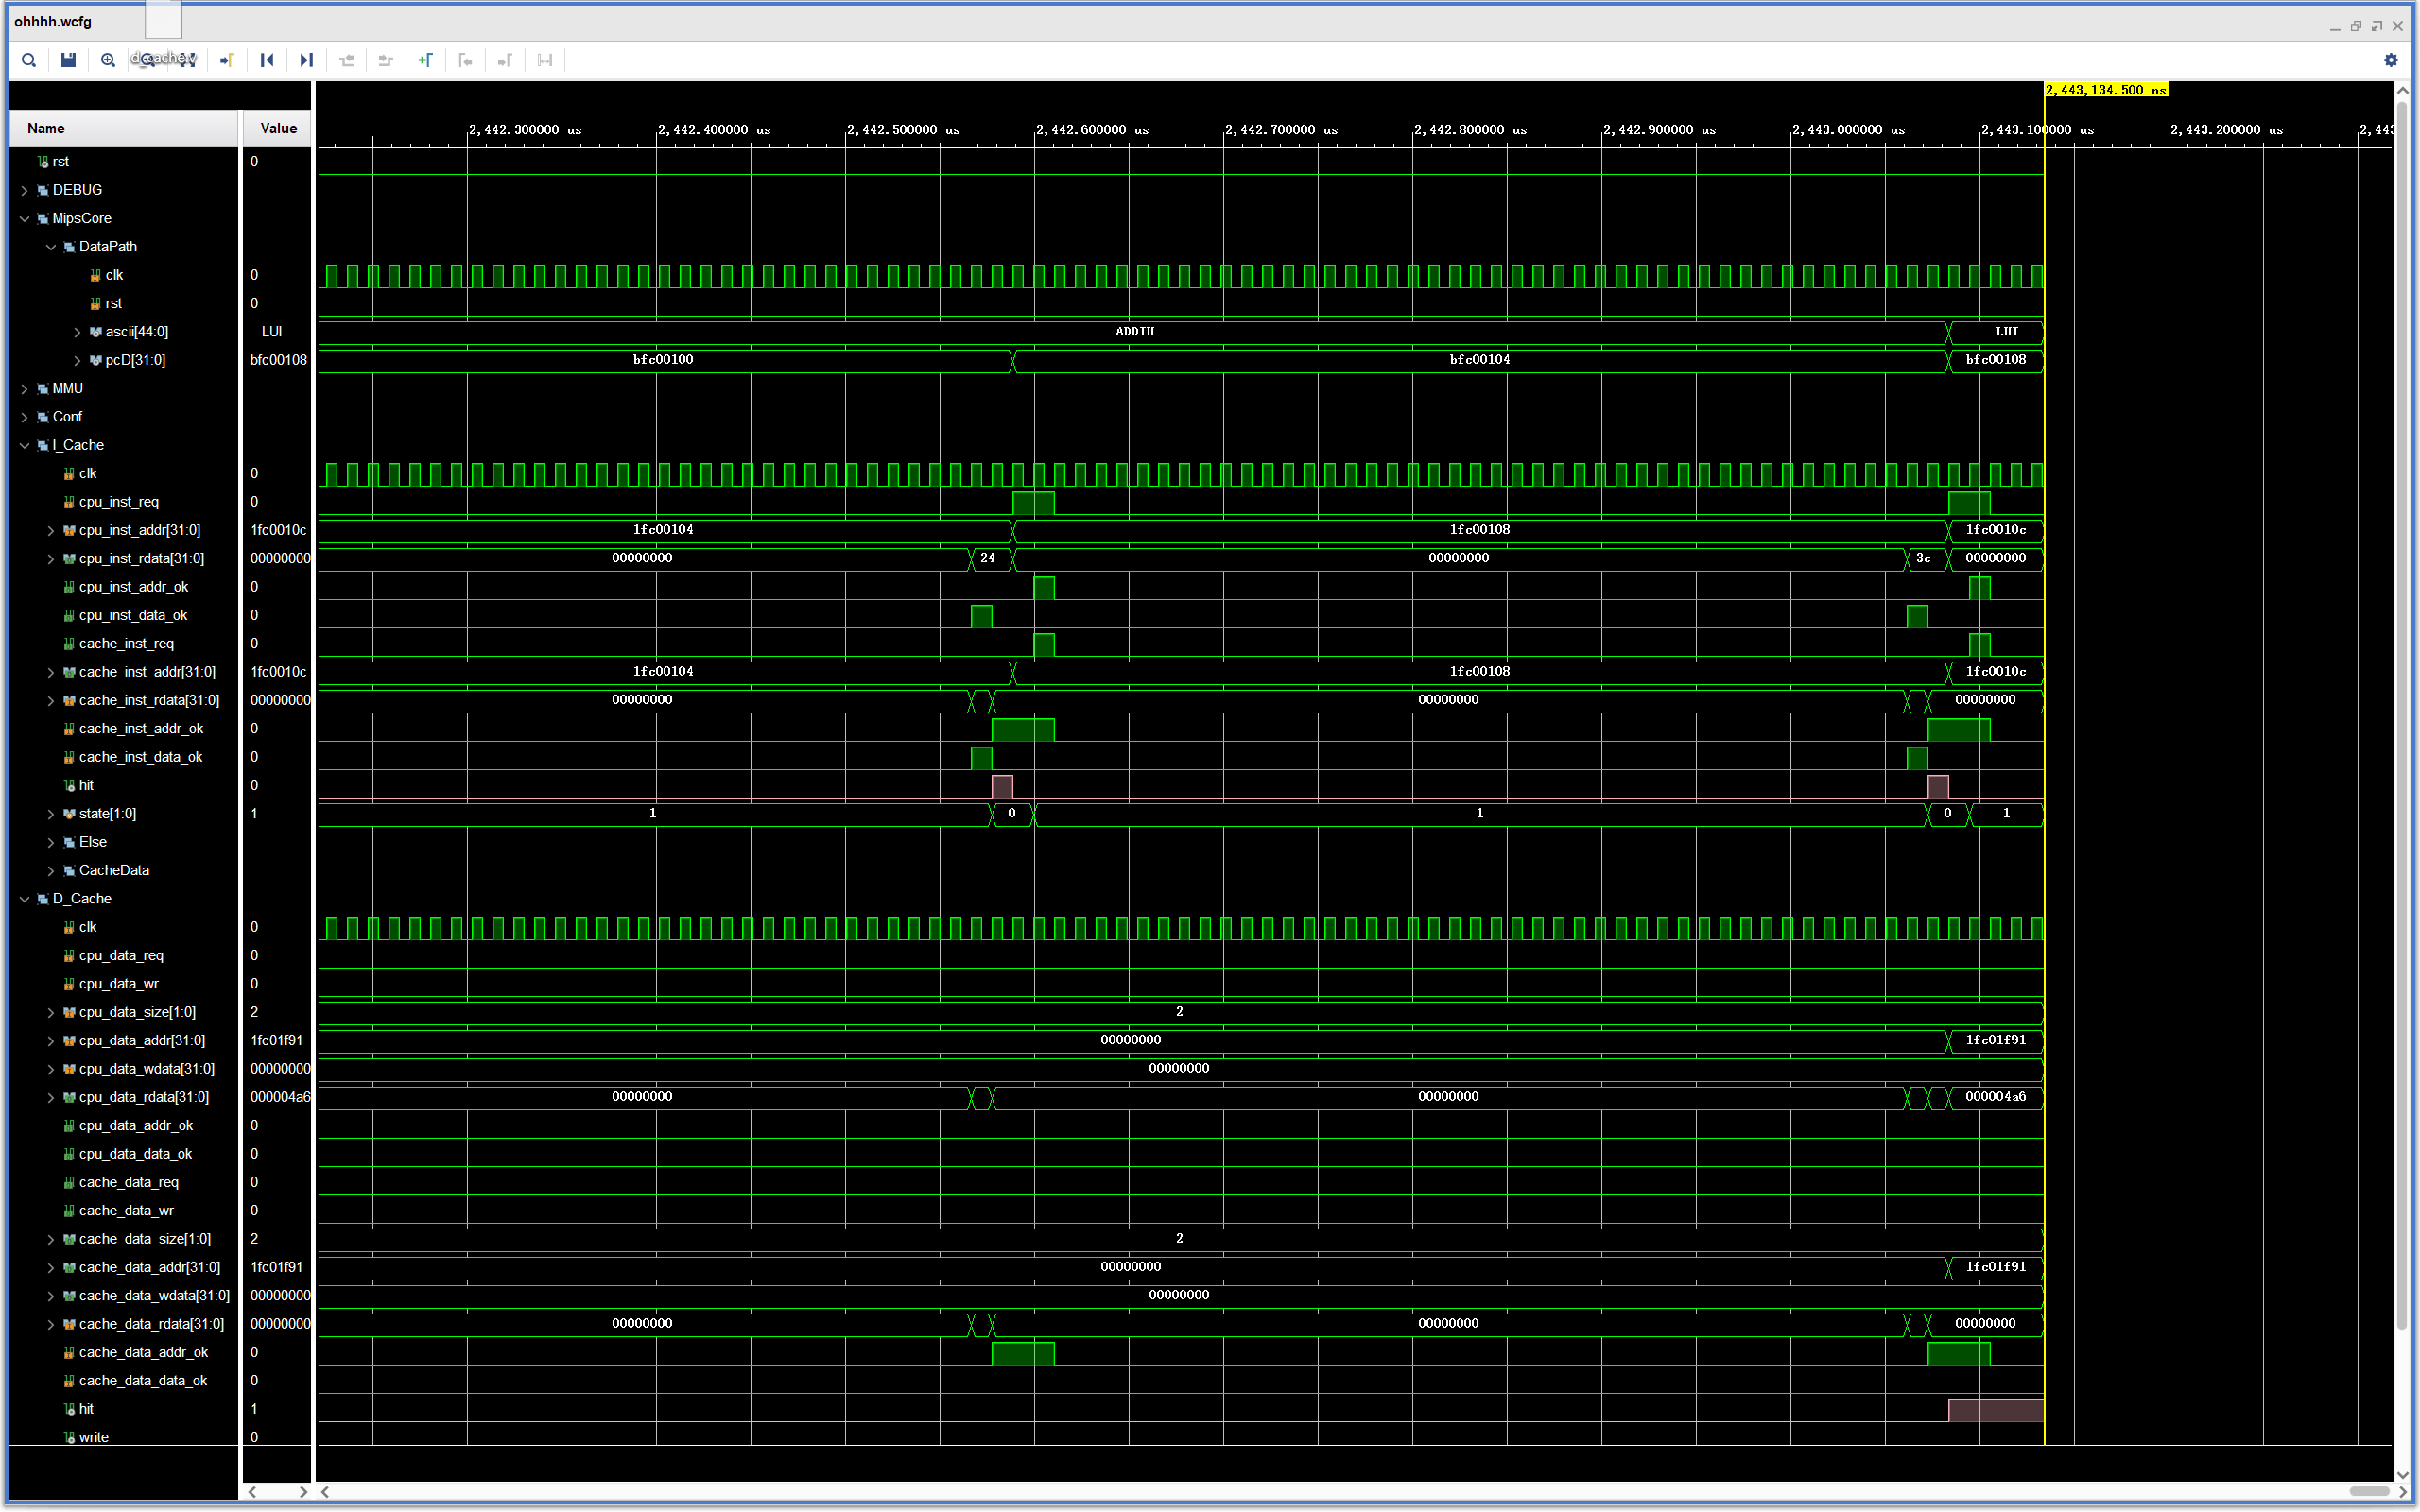
\includegraphics[width=\textwidth]{image/wt.png}
    \caption{写直达}
    \label{fig:sub-a}
  \end{subfigure}
  \hfill
  \begin{subfigure}[b]{0.6\textwidth}
    \centering
    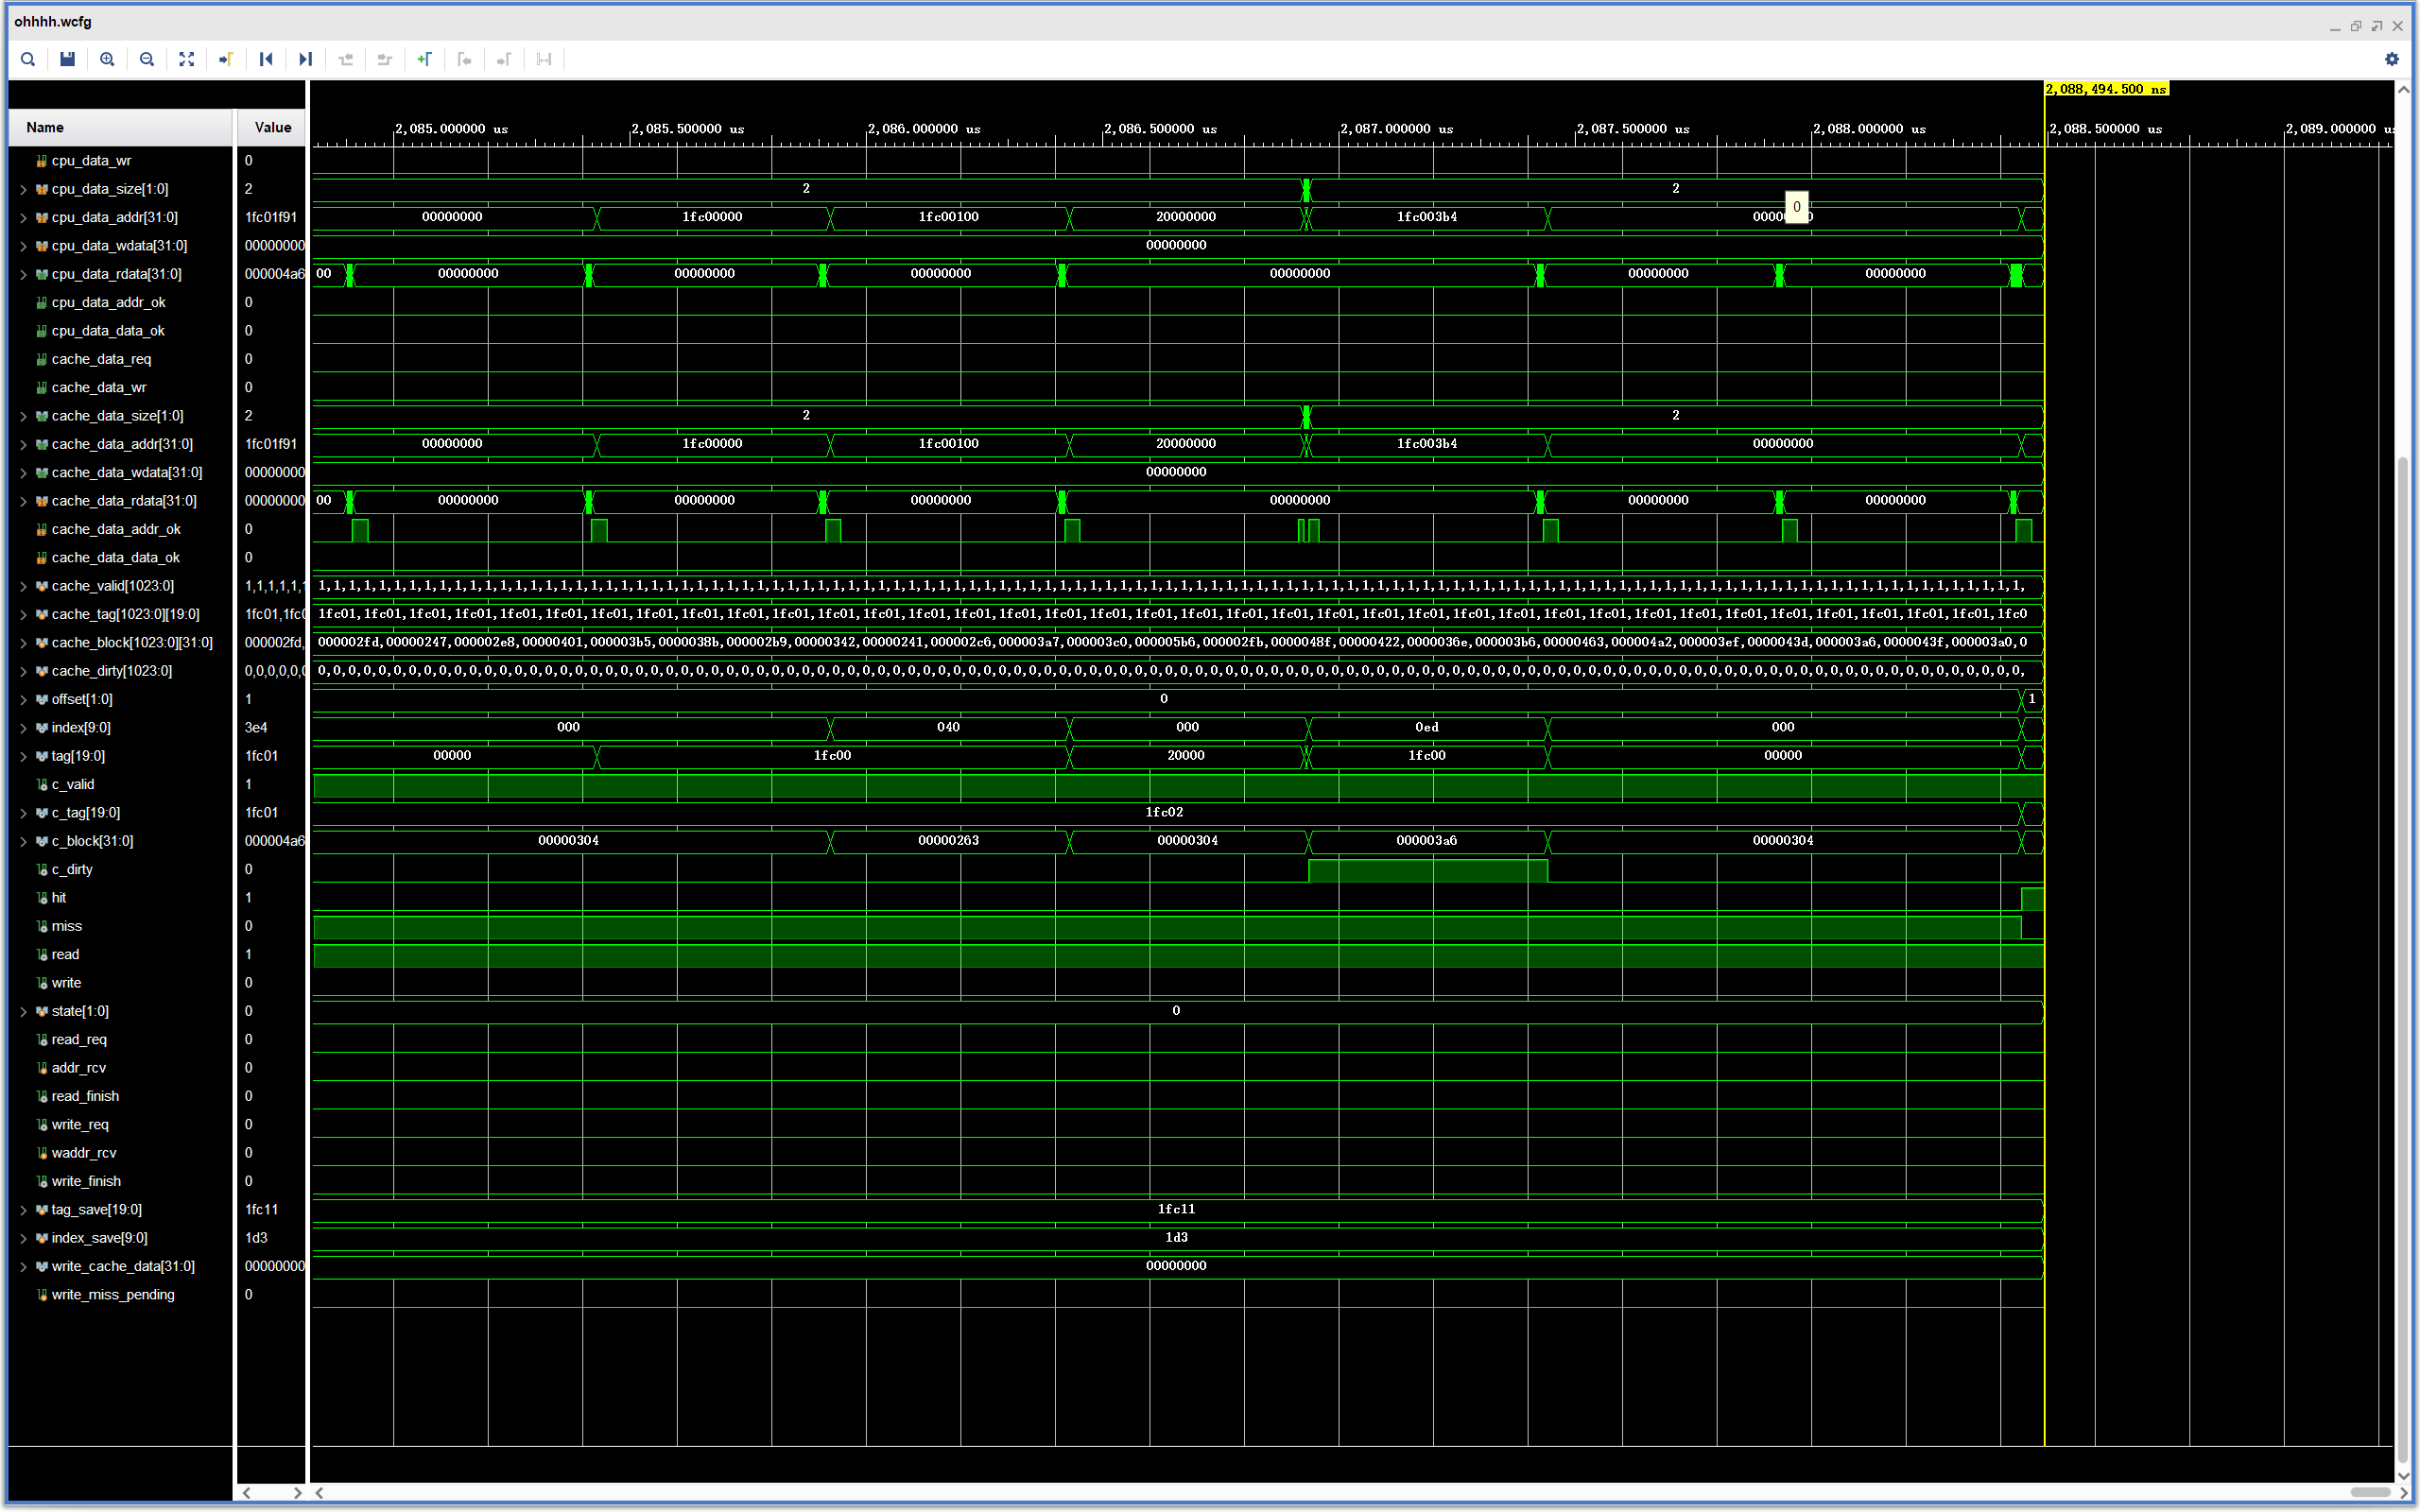
\includegraphics[width=\textwidth]{image/wb.png}
    \caption{写回-写分配}
    \label{fig:sub-b}
  \end{subfigure}

  \caption{写直达和写回-写分配的仿真对比}
  \label{fig:sim_compare}
\end{figure}
\begin{figure}[H]
    \centering
    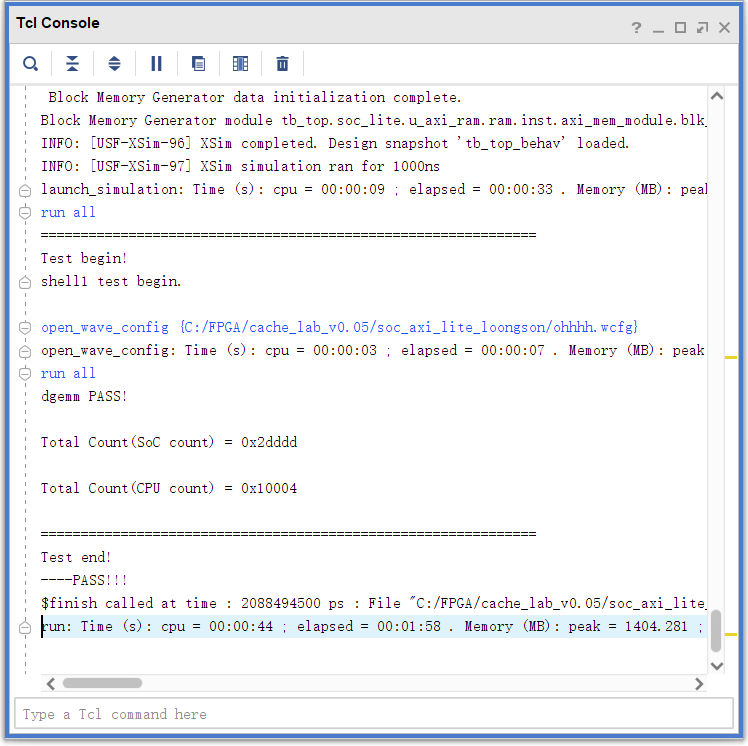
\includegraphics[width=0.9\textwidth]{image/pass.png}
    \caption{通过仿真测试}
    \label{fig:tcl}
\end{figure}